\documentclass[12pt]{report}
\usepackage[utf8]{inputenc}
\usepackage[english, russian]{babel}
\usepackage{listings}
\usepackage{graphicx}
\usepackage{float}
\graphicspath{{imgs/}}
\usepackage{amsmath,amsfonts,amssymb,amsthm,mathtools} 
\usepackage{pgfplots}
\usepackage{filecontents}
\usepackage{indentfirst}
\usepackage{eucal}
\usepackage{enumitem}
\frenchspacing

\usepackage{indentfirst} % Красная строка

\usetikzlibrary{datavisualization}
\usetikzlibrary{datavisualization.formats.functions}

\usepackage{amsmath}
\usepackage{fixltx2e}
\usepackage{caption}


\definecolor{bluekeywords}{rgb}{0,0,1}
\definecolor{greencomments}{rgb}{0,0.5,0}
\definecolor{redstrings}{rgb}{0.64,0.08,0.08}
\definecolor{xmlcomments}{rgb}{0.5,0.5,0.5}
\definecolor{types}{rgb}{0.17,0.57,0.68}

\usepackage{listings}
\usepackage{listingsutf8}
\usepackage{xcolor}
\lstset{language=Matlab,%
	%basicstyle=\color{red},
	breaklines=true,%
	frame=single, % Oberhalb und unterhalb des Listings ist eine Linie
	morekeywords={matlab2tikz},
	keywordstyle=\color{blue},%
	morekeywords=[2]{1}, keywordstyle=[2]{\color{black}},
	identifierstyle=\color{black},%
	stringstyle=\color{red},
	commentstyle=\color{black},%
	showstringspaces=false,%without this there will be a symbol in the places where there is a space
	numbers=left,%
	numberstyle={\tiny \color{black}},% size of the numbers
	numbersep=9pt, % this defines how far the numbers are from the text
	emph=[1]{for,end,break},emphstyle=[1]\color{red}, %some words to emphasise
	%emph=[2]{word1,word2}, emphstyle=[2]{style},    
	literate={Ö}{{\"O}}1
	{Ä}{{\"A}}1
	{Ü}{{\"U}}1
	{ß}{{\ss}}1
	{ü}{{\"u}}1
	{ä}{{\"a}}1
	{ö}{{\"o}}1
	{~}{{\textasciitilde}}1
	{а}{{\selectfont\char224}}1
	{б}{{\selectfont\char225}}1
	{в}{{\selectfont\char226}}1
	{г}{{\selectfont\char227}}1
	{д}{{\selectfont\char228}}1
	{е}{{\selectfont\char229}}1
	{ё}{{\"e}}1
	{ж}{{\selectfont\char230}}1
	{з}{{\selectfont\char231}}1
	{и}{{\selectfont\char232}}1
	{й}{{\selectfont\char233}}1
	{к}{{\selectfont\char234}}1
	{л}{{\selectfont\char235}}1
	{м}{{\selectfont\char236}}1
	{н}{{\selectfont\char237}}1
	{о}{{\selectfont\char238}}1
	{п}{{\selectfont\char239}}1
	{р}{{\selectfont\char240}}1
	{с}{{\selectfont\char241}}1
	{т}{{\selectfont\char242}}1
	{у}{{\selectfont\char243}}1
	{ф}{{\selectfont\char244}}1
	{х}{{\selectfont\char245}}1
	{ц}{{\selectfont\char246}}1
	{ч}{{\selectfont\char247}}1
	{ш}{{\selectfont\char248}}1
	{щ}{{\selectfont\char249}}1
	{ъ}{{\selectfont\char250}}1
	{ы}{{\selectfont\char251}}1
	{ь}{{\selectfont\char252}}1
	{э}{{\selectfont\char253}}1
	{ю}{{\selectfont\char254}}1
	{я}{{\selectfont\char255}}1
	{А}{{\selectfont\char192}}1
	{Б}{{\selectfont\char193}}1
	{В}{{\selectfont\char194}}1
	{Г}{{\selectfont\char195}}1
	{Д}{{\selectfont\char196}}1
	{Е}{{\selectfont\char197}}1
	{Ё}{{\"E}}1
	{Ж}{{\selectfont\char198}}1
	{З}{{\selectfont\char199}}1
	{И}{{\selectfont\char200}}1
	{Й}{{\selectfont\char201}}1
	{К}{{\selectfont\char202}}1
	{Л}{{\selectfont\char203}}1
	{М}{{\selectfont\char204}}1
	{Н}{{\selectfont\char205}}1
	{О}{{\selectfont\char206}}1
	{П}{{\selectfont\char207}}1
	{Р}{{\selectfont\char208}}1
	{С}{{\selectfont\char209}}1
	{Т}{{\selectfont\char210}}1
	{У}{{\selectfont\char211}}1
	{Ф}{{\selectfont\char212}}1
	{Х}{{\selectfont\char213}}1
	{Ц}{{\selectfont\char214}}1
	{Ч}{{\selectfont\char215}}1
	{Ш}{{\selectfont\char216}}1
	{Щ}{{\selectfont\char217}}1
	{Ъ}{{\selectfont\char218}}1
	{Ы}{{\selectfont\char219}}1
	{Ь}{{\selectfont\char220}}1
	{Э}{{\selectfont\char221}}1
	{Ю}{{\selectfont\char222}}1
	{Я}{{\selectfont\char223}}1
	{і}{{\selectfont\char105}}1
	{ї}{{\selectfont\char168}}1
	{є}{{\selectfont\char185}}1
	{ґ}{{\selectfont\char160}}1
	{І}{{\selectfont\char73}}1
	{Ї}{{\selectfont\char136}}1
	{Є}{{\selectfont\char153}}1
	{Ґ}{{\selectfont\char128}}1
}

\usepackage[left=1cm,right=1cm, top=1cm,bottom=1.5cm,bindingoffset=0cm]{geometry}
% Для измененных титулов глав:
\usepackage{titlesec, blindtext, color} % подключаем нужные пакеты
\definecolor{gray75}{gray}{0.75} % определяем цвет
\newcommand{\hsp}{\hspace{20pt}} % длина линии в 20pt
% titleformat определяет стиль
\titleformat{\chapter}[hang]{\Huge\bfseries}{\thechapter\hsp\textcolor{gray75}{|}\hsp}{0pt}{\Huge\bfseries}

\usepackage{array}
\newcommand{\head}[2]{\multicolumn{1}{>{\centering\arraybackslash}p{#1}}{#2}}

% plot
\usepackage{pgfplots}
\usepackage{filecontents}
\usetikzlibrary{datavisualization}
\usetikzlibrary{datavisualization.formats.functions}

\begin{document}
	%\def\chaptername{} % убирает "Глава"
	\thispagestyle{empty}
	\begin{titlepage}
		\noindent \begin{minipage}{0.15\textwidth}
			
\includegraphics[width=\linewidth]{b_logo}
		\end{minipage}
		\noindent\begin{minipage}{0.9\textwidth}\centering
			\textbf{Министерство науки и высшего образования Российской Федерации}\\
			\textbf{Федеральное государственное бюджетное образовательное учреждение высшего образования}\\
			\textbf{~~~«Московский государственный технический университет имени Н.Э.~Баумана}\\
			\textbf{(национальный исследовательский университет)»}\\
			\textbf{(МГТУ им. Н.Э.~Баумана)}
		\end{minipage}
		
		\noindent\rule{18cm}{3pt}
		\newline\newline
		\noindent ФАКУЛЬТЕТ $\underline{\text{«Информатика и системы управления»}}$ \newline\newline
		\noindent КАФЕДРА $\underline{\text{«Программное обеспечение ЭВМ и информационные технологии»}}$\newline\newline\newline\newline\newline\newline\newline\newline\newline\newline\newline
		
		
		\begin{center}
			\noindent\begin{minipage}{1.3\textwidth}\centering
				\Large\textbf{  Отчет по лабораторной работе №2}\newline
				\textbf{по дисциплине \newline "Математическая статистика"}\newline\newline
			\end{minipage}
		\end{center}
		
		\noindent\textbf{Тема} $\underline{\text{Интервальные оценки}}$\newline\newline
		\noindent\textbf{Студент} $\underline{\text{Малышев И. А.}}$\newline\newline
		\noindent\textbf{Группа} $\underline{\text{ИУ7-61Б}}$\newline\newline
		\noindent\textbf{Оценка (баллы)} $\underline{\text{~~~~~~~~~~~~~~~~~~~~~~~~~~~}}$\newline\newline
		\noindent\textbf{Преподаватель: } $\underline{\text{Власов П. А.}}$\newline\newline\newline
		
		\begin{center}
			\vfill
			Москва~---~\the\year
			~г.
		\end{center}
	\end{titlepage}
	
\setcounter{page}{2}

\chapter*{Задание}

\section*{Цель работы}
Построение доверительных интервалов для математического ожидания и дисперсии нормальной случайной величины.

\section*{Постановка задачи}

\begin{enumerate}
	\setlength\itemsep{0.01em}
	\item Для выборки объема $n$ из нормальной генеральной совокупности $X$ реализовать в виде программы на ЭВМ
	\begin{enumerate}
		\setlength\itemsep{0.01em}
		\item вычисление точечных оценок $\hat\mu(\vec X_n)$ и $S^2(\vec X_n)$ математического ожидания $MX$ и дисперсии $DX$ соответственно;
		\item вычисление нижней и верхней границ $\underline\mu(\vec X_n)$, $\overline\mu(\vec X_n)$ для $\gamma$-доверительного интервала для математического ожидания $MX$;
		\item вычисление нижней и верхней границ $\underline\sigma^2(\vec X_n)$, $\overline\sigma^2(\vec X_n)$ для $\gamma$-доверительного интервала для дисперсии $DX$;
	\end{enumerate}
	\item вычислить $\hat\mu$ и $S^2$ для выборки из индивидуального варианта;
	\item для заданного пользователем уровня доверия $\gamma$ и $N$ – объёма выборки из индивидуального варианта:
	\begin{enumerate}
		\setlength\itemsep{0.01em}
		\item на координатной плоскости $Oyn$ построить прямую $y = \hat\mu(\vec{x_N})$, также графики функций $y = \hat\mu(\vec x_n)$, $y = \underline\mu(\vec x_n)$ и $y = \overline\mu(\vec x_n)$ как функций объема $n$ выборки, где $n$ изменяется от 1 до $N$;
		\item на другой координатной плоскости $Ozn$ построить прямую $z = S^2(\vec{x_N})$, также графики функций $z = S^2(\vec x_n)$, $z = \underline\sigma^2(\vec x_n)$ и $z = \overline\sigma^2(\vec x_n)$ как функций объема $n$ выборки, где $n$ изменяется от 1 до $N$.
	\end{enumerate}
\end{enumerate}

\section*{Вариант выборки}
Вариант 13

$\vec{X}$=(-10.82,-9.27,-9.65,-9.36,-9.27,-11.25,-9.89,-9.26,-11.15,-8.90,-11.02,-8.28,-9.18,-10.16,-10.59,-10.82,-9.05,-9.47,-10.98,-11.50,-8.64,-10.86,-10.76,-11.49,-11.09,-9.33,-9.32,-9.66,-8.79,-10.54,-9.12,-10.40,-8.59,-10.22,-9.06,-10.59,-10.60,-10.25,-9.35,-11.44,-9.81,-9.32,-9.95,-9.33,-10.64,-9.45,-10.99,-10.15,-10.39,-10.36,-10.49,-11.67,-10.00,-10.87,-11.11,-9.68,-10.77,-9.13,-8.62,-10.33,-11.36,-10.24,-9.41,-11.05,-10.15,-9.35,-11.45,-9.87,-10.41,-10.11,-10.84,-11.48,-7.77,-10.79,-9.88,-10.70,-9.07,-9.47,-10.15,-9.93,-11.52,-9.04,-10.93,-10.13,-9.56,-11.39,-9.79,-9.19,-11.09,-9.86,-10.67,-10.26,-9.07,-10.53,-11.24,-10.16,-11.33,-8.76,-8.88,-10.53,-10.12,-8.98,-9.84,-9.90,-10.13,-9.32,-9.31,-9.99,-8.55,-11.64,-11.32,-10.51,-11.71,-10.50,-10.50,-12.20,-11.68,-10.45,-7.88,-10.84)

\chapter*{Теоретические сведения}

\section*{Определение $\gamma$-доверительного интервала для значения параметра распределения случайной величины}

Дана случайная величина $X$, закон распределения которой известен с точностью до неизвестного параметра $\theta$.

Интервальной оценкой с уровнем доверия $\gamma$ ($\gamma$-доверительной интервальной оценкой) параметра $\theta$ называют пару статистик $\underline{\theta}(\vec X), \overline{\theta}(\vec X)$ таких, что

\begin{equation*}
	P\{\underline{\theta}(\vec X)<\theta<\overline{\theta}(\vec X)\}=\gamma
\end{equation*}

Поскольку границы интервала являются случайными величинами, то для различных реализаций случайной выборки $\vec X$ статистики $\underline{\theta}(\vec X), \overline{\theta}(\vec X)$ могут принимать различные значения.

Доверительным интервалом с уровнем доверия $\gamma$ ($\gamma$-доверительным интервалом) называют интервал $(\underline{\theta}(\vec x), \overline{\theta}(\vec x))$, отвечающий выборочным значениям статистик $\underline{\theta}(\vec X), \overline{\theta}(\vec X)$.

\section*{Формулы для вычисления границ $\gamma$-доверительного интервала для математического ожидания и дисперсии нормальной случайной величины}

Формулы для вычисления границ $\gamma$-доверительного интервала для математического ожидания:

\begin{equation}
	\underline\mu(\vec X_n)=\overline X + \frac{S(\vec X)t^{St(n-1)}_{\frac{1-\gamma}{2}}}{\sqrt{n}}
\end{equation}

\begin{equation}
	\overline\mu(\vec X_n)=\overline X + \frac{S(\vec X)t^{St(n-1)}_{\frac{1+\gamma}{2}}}{\sqrt{n}}
\end{equation}

$\overline X$ -- выборочное среднее;

$S(\vec X) = \sqrtsign{S^2(\vec X)}$ -- квадратный корень из исправленной выборочной дисперсии;

$n$ -- объем выборки;

$\gamma$ -- уровень доверия;

$t^{St(n-1)}_{\alpha}$ -- квантиль уровня $\alpha$ распределения Стьюдента с $n - 1$ степенями свободы.

Формулы для вычисления границ $\gamma$-доверительного интервала для дисперсии:

\begin{equation}
	\underline\sigma(\vec X_n)= \sqrt{\frac{(n-1)S^2(\vec X)}{t^{\chi^2(n-1)}_{\frac{1+\gamma}{2}}}}
\end{equation}

\begin{equation}
	\overline\sigma(\vec X_n)= \sqrt{\frac{(n-1)S^2(\vec X)}{t^{\chi^2(n-1)}_{\frac{1-\gamma}{2}}}}
\end{equation}

$S^2(\vec X)$ -- исправленная выборочная дисперсия;

$n$ -- объем выборки;

$\gamma$ -- уровень доверия;

$t^{\chi^2(n-1)}_{\alpha}$ -- квантиль уровня $\alpha$ распределения $\chi^2(n-1)$ с $n - 1$ степенями свободы.


\chapter*{Результаты работы программы}

\section*{Текст программы}
\begin{lstlisting}[mathescape]
function main()
	X = [-10.82,-9.27,-9.65,-9.36,-9.27,-11.25,-9.89,-9.26,-11.15,-8.90, -11.02,-8.28,-9.18,-10.16,-10.59,-10.82,-9.05,-9.47,-10.98,-11.50,
	-8.64,-10.86,-10.76,-11.49,-11.09,-9.33,-9.32,-9.66,-8.79,-10.54,-9.12,
	-10.40,-8.59,-10.22,-9.06,-10.59,-10.60,-10.25,-9.35,-11.44,-9.81,
	-9.32,-9.95,-9.33,-10.64,-9.45,-10.99,-10.15,-10.39,-10.36,-10.49,
	-11.67,-10.00,-10.87,-11.11,-9.68,-10.77,-9.13,-8.62,-10.33,-11.36,
	-10.24,-9.41,-11.05,-10.15,-9.35,-11.45,-9.87,-10.41,-10.11,-10.84,
	-11.48,-7.77,-10.79,-9.88,-10.70,-9.07,-9.47,-10.15,-9.93,-11.52,-9.04,
	-10.93,-10.13,-9.56,-11.39,-9.79,-9.19,-11.09,-9.86,-10.67,-10.26,
	-9.07,-10.53,-11.24,-10.16,-11.33,-8.76,-8.88,-10.53,-10.12,-8.98,
	-9.84,-9.90,-10.13,-9.32,-9.31,-9.99,-8.55,-11.64,-11.32,-10.51,-11.71,
	-10.50,-10.50,-12.20,-11.68,-10.45,-7.88,-10.84];

    % Уровень доверия
	gamma = 0.9;
	% Объем выборки 
	n = length(X);
	% Точечная оценка мат. ожидания
	mu = mean(X);
	% Точечная оценка дисперсии
	s2 = var(X);
	
	% Нижняя граница доверительного интервала для мат. ожидания
	muBot = findMuBot(n, mu, s2, gamma);
	% Верхняя граница доверительного интервала для мат. ожидания
	muTop = findMuTop(n, mu, s2, gamma);
	% Нижняя граница доверительного интервала для дисперсии
	s2Bot = findS2Bot(n, s2, gamma);
	% Верхняя граница доверительного интервала для дисперсии
	s2Top = findS2Top(n, s2, gamma);
	
	% Вывод полученных ранее значений
	fprintf('$\mu$ (Выборочное среднее) = %.3f\n', mu);
	fprintf('S^2 (Исправленная выборочная дисперсия) = %.3f\n', s2);
	fprintf('$\mu$_Bot (нижняя граница доверительного интервала для математического ожидания) = %.3f\n', muBot);
	fprintf('$\mu$_Top (верхняя граница доверительного интервала для математического ожидания) = %.3f\n', muTop);
	fprintf('S^2_Bot (нижняя граница доверительного интервала для дисперсии) = %.3f\n', s2Bot);
	fprintf('S^2_Top (верхняя граница доверительного интервала для дисперсии) = %.3f\n', s2Top);
	
	% Создание массивов точечных оценок
	muArray = zeros(1, n);
	s2Array = zeros(1, n);
	% Создание массивов границ доверительных интервалов
	muBotArray = zeros(1, n);
	muTopArray = zeros(1, n);
	s2BotArray = zeros(1, n);
	s2TopArray = zeros(1, n);
	
	for i = 1 : n
		mu = mean(X(1:i));
		s2 = var(X(1:i));
		% Точечная оценка матожидания
		muArray(i) = mu;
		% Точечная оценка дисперсии
		s2Array(i) = s2;
		% Нижняя граница доверительного интервала для матожидания
		muBotArray(i) = findMuBot(i, mu, s2, gamma);
		% Верхняя граница доверительного интервала для матожидания
		muTopArray(i) = findMuTop(i, mu, s2, gamma);
		% Нижняя граница доверительного интервала для дисперсии
		s2BotArray(i) = findS2Bot(i, s2, gamma);
		% Верхняя граница доверительного интервала для дисперсии
		s2TopArray(i) = findS2Top(i, s2, gamma);
	end
	
	% Построение графиков
	plot(1 : n, [(zeros(1, n) + mu)', muArray', muBotArray', muTopArray']);
	xlabel('n');
	ylabel('y');
	legend('$\hat \mu(\vec x_N)$', '$\hat \mu(\vec x_n)$', ...
	'$\underline{\mu}(\vec x_n)$', '$\overline{\mu}(\vec x_n)$', ...
	'Interpreter', 'latex', 'FontSize', 18);
	figure;
	plot(1 : n, [(zeros(1, n) + s2)', s2Array', s2BotArray', s2TopArray']);
	xlabel('n');
	ylabel('z');
	legend('$\hat S^2(\vec x_N)$', '$\hat S^2(\vec x_n)$', ...
	'$\underline{\sigma}^2(\vec x_n)$', '$\overline{\sigma}^2(\vec x_n)$', ...
	'Interpreter', 'latex', 'FontSize', 18);
end

% Функция поиска нижней границы доверительного интервала для матожидания
function muBot = findMuBot(n, mu, s2, gamma)
	muBot = mu - sqrt(s2) * tinv((1 + gamma) / 2, n - 1) / sqrt(n);
end

% Функция поиска верхней границы доверительного интервала для матожидания
function muTop = findMuTop(n, mu, s2, gamma)
	muTop = mu + sqrt(s2) * tinv((1 + gamma) / 2, n - 1) / sqrt(n);
end

% Функция поиска нижней границы доверительного интервала для дисперсии
function s2Bot = findS2Bot(n, s2, gamma)
	s2Bot = ((n - 1) * s2) / chi2inv((1 + gamma) / 2, n - 1);
end

% Функция поиска верхней границы доверительного интервала для дисперсии
function s2Top = findS2Top(n, s2, gamma)
	s2Top = ((n - 1) * s2) / chi2inv((1 - gamma) / 2, n - 1);
end

\end{lstlisting}

\section*{Результаты расчётов}

\begin{itemize}
	\item $\mu$ (Выборочное среднее) = -10.132
	\item $S^2$ (Исправленная выборочная дисперсия) = 0.846
	\item $\underline{\mu}$ (нижняя граница доверительного интервала для математического ожидания) = -10.271
	\item $\overline{\mu}$ (верхняя граница доверительного интервала для математического ожидания) = -9.993
	\item $\underline{S^2}$ (нижняя граница доверительного интервала для дисперсии) = 0.692
	\item $\overline{S^2}$ (верхняя граница доверительного интервала для дисперсии) = 1.062
\end{itemize}

\begin{figure}[H]
	\centering
	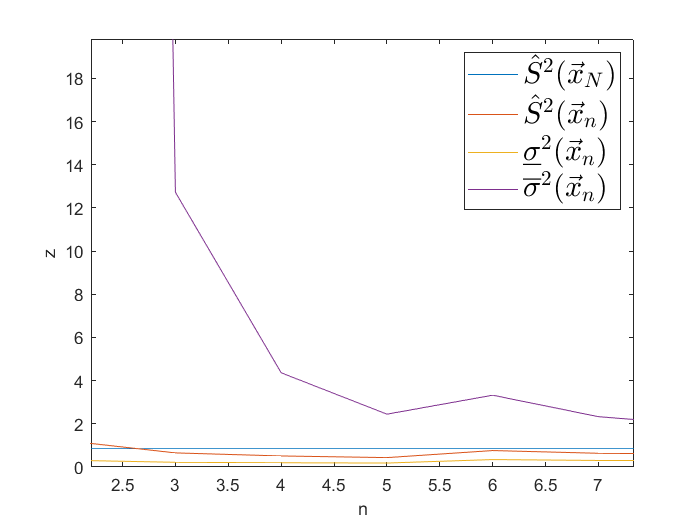
\includegraphics[scale=0.7]{imgs/1.png}
	\caption{Прямая $z=\hat S^2 (\vec x_N)$ и графики функций $z= S^2 (\vec x_n), z= \underline \sigma^2 (\vec x_n), z =\overline \sigma^2 (\vec x_n)$ как функций объема n выборки, где n изменяется от 1 до N.}
	\label{fig:1}
\end{figure}

\begin{figure}[H]
	\centering
	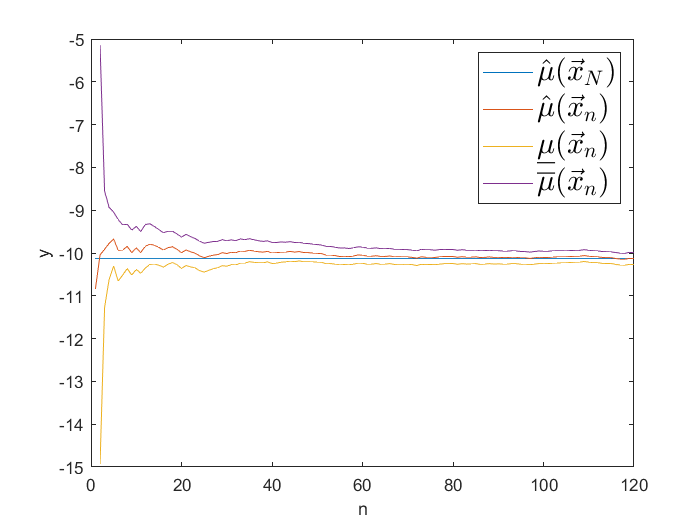
\includegraphics[scale=0.7]{imgs/2.png}
	\caption{Прямая $y=\hat \mu (\vec x_N)$ и графики функций $y=\hat \mu (\vec x_n), y= \underline \mu (\vec x_n), y =\overline \mu (\vec x_n)$ как функций объема n выборки, где n изменяется от 1 до N.}
	\label{fig:2}
\end{figure}

\end{document}